%\VignetteIndexEntry{Answers to Exercise 01 from Seminar III: R/Bioconductor}
%\VignetteDepends{}
%\VignetteKeywords{R, Bioconductor}
%\VignettePackage{SIII: R/Bioc}
\documentclass[letterpaper,12pt]{article}

%%%%%%%%%%%%%%%%%%%%%%%% Standard Packages %%%%%%%%%%%%%%%%%%%%%%%%%%%%%%%%%%%%%%%%%%
\usepackage{fancyvrb}
\usepackage{fancyhdr}

\usepackage[a4paper]{geometry}
\usepackage{hyperref,graphicx}

% Un-comment the next 3 lines to use spanish symbols such as accents
%\usepackage[spanish]{babel}
%\selectlanguage{spanish}
%\usepackage[utf8]{inputenc}

%%%%%%%%%%%%%%%%%%%%%% some personal commands %%%%%%%%%%%%%%%%%%%%%%%%%%%%%%%%%%%%%%%%%%%%
\newcommand{\pl}[1]{\texttt{#1}}
\newcommand{\myurlshort}[2]{\href{http://#1}{{\textsf{#2}}}}

%%%%%%%%%%%%%%%%%%%%%% headers and footers %%%%%%%%%%%%%%%%%%%%%%%%%%%%%%%%%%%%%%%%%%%%
\pagestyle{fancy} 
\renewcommand{\footrulewidth}{\headrulewidth}

%%%%%%%%%%%%%%%%%%%%%%%%% bibliography  %%%%%%%%%%%%%%%%%%%%%%%%%%%%%%%%%%%%%%%%%%%%%%%
\bibliographystyle{plainnat}

%%%%%%%%%%%%%%%%%%%%%%%%% sweave options  %%%%%%%%%%%%%%%%%%%%%%%%%%%%%%%%%%%%%%%%%%%%%%%



%%%%%%%%%%%%%%%%%%%%%%% opening %%%%%%%%%%%%%%%%%%%%%%%%%%%%%%%%%%%%
\title{\textbf{Seminar III: \texttt{R}/\texttt{Bioconductor}\\ \small August-December 2009}}
\author{Leonardo Collado Torres\\[1em]Bachelor in Genomic Sciences (LCG),\\ UNAM, Cuernavaca, Mexico\\[1em]\texttt{lcollado@lcg.unam.mx}\\[1em]\url{http://www.lcg.unam.mx/~lcollado/}}

\usepackage{Sweave}
\begin{document}
\maketitle

\medskip
\noindent{\small\textbf{Assistants:} Alejandro Reyes \pl{areyes@lcg.unam.mx}, Jos\'e Reyes \pl{jreyes@lcg.unam.mx} and V\'ictor Moreno \pl{jmoreno@lcg.unam.mx}}

\medskip
\noindent{\small\textbf{Note:} Questions through the \myurlshort{foros.nnb.unam.mx/viewforum.php?f=111}{forum} please. Those who are not from the sixth LCG generation send us an email so we can register you on the forum.}

\medskip
\begin{abstract}
Expected solutions to the first set of exercises.
\end{abstract}

\section{Review}
  \begin{enumerate}
  \item Why does the following expression show a warning? This is part of what rule?
\begin{Schunk}
\begin{Sinput}
> c(2, 3) + c(4, 5, 7)
\end{Sinput}
\end{Schunk}
\begin{Schunk}
\begin{Sinput}
> "Because the 2nd vector's length is not a multiple of the first one"
\end{Sinput}
\begin{Soutput}
[1] "Because the 2nd vector's length is not a multiple of the first one"
\end{Soutput}
\begin{Sinput}
> "and viceversa. Its due to the recycling rule."
\end{Sinput}
\begin{Soutput}
[1] "and viceversa. Its due to the recycling rule."
\end{Soutput}
\end{Schunk}
  \item For all the prime numbers between 1 and 10, calculate its square root. What is the sum, median and mean?
\begin{Schunk}
\begin{Sinput}
> prime <- c(2, 3, 5, 7)
> sqrt(prime)
\end{Sinput}
\begin{Soutput}
[1] 1.414214 1.732051 2.236068 2.645751
\end{Soutput}
\begin{Sinput}
> sum(prime)
\end{Sinput}
\begin{Soutput}
[1] 17
\end{Soutput}
\begin{Sinput}
> sum(sqrt(prime))
\end{Sinput}
\begin{Soutput}
[1] 8.028084
\end{Soutput}
\begin{Sinput}
> median(prime)
\end{Sinput}
\begin{Soutput}
[1] 4
\end{Soutput}
\begin{Sinput}
> median(sqrt(prime))
\end{Sinput}
\begin{Soutput}
[1] 1.984059
\end{Soutput}
\begin{Sinput}
> mean(prime)
\end{Sinput}
\begin{Soutput}
[1] 4.25
\end{Soutput}
\begin{Sinput}
> mean(sqrt(prime))
\end{Sinput}
\begin{Soutput}
[1] 2.007021
\end{Soutput}
\end{Schunk}
  \end{enumerate}

\section{Plots}
  \begin{itemize}
  \item Read the following file into \pl{R}: \url{ftp://ftp.ebi.ac.uk/pub/databases/genome_reviews/gr2species_phage.txt}\footnote{Look for the useful function for this case} and make the following plots with your username on the title. Check whether using a log10 scale on the $y$ axis helps.
\begin{Schunk}
\begin{Sinput}
> phage <- read.delim(file.path("ftp://ftp.ebi.ac.uk/pub/databases/genome_reviews/gr2species_phage.txt"), 
+     header = F)
\end{Sinput}
\end{Schunk}
  \begin{enumerate}
  \item Sort the genome sizes (column 2) and plot them in a line with increasing values.
\begin{Schunk}
\begin{Sinput}
> plot(sort(phage[, 2]), type = "l", 
+     col = "blue", main = "lcollado")
\end{Sinput}
\end{Schunk}
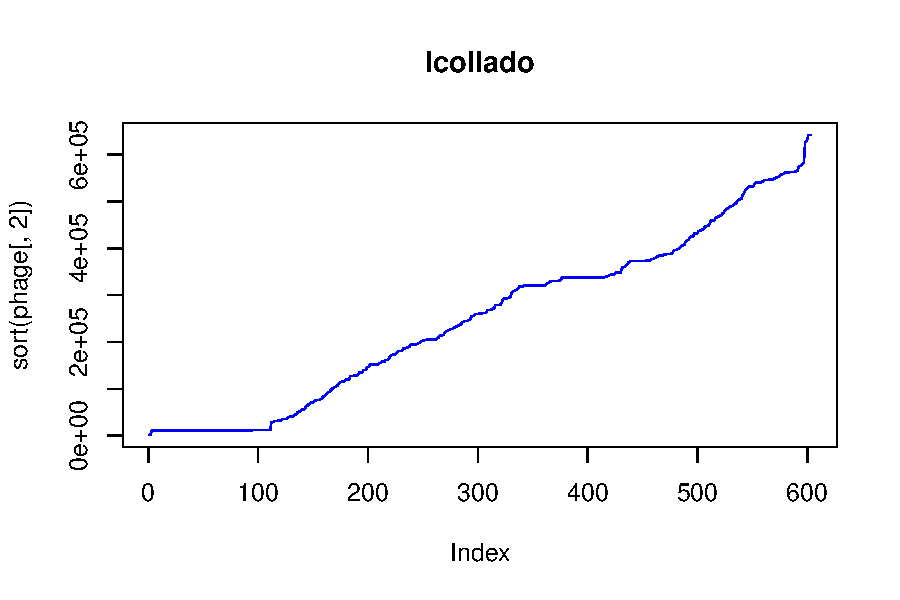
\includegraphics{plots/fig-006}
\begin{Schunk}
\begin{Sinput}
> plot(sort(log10(phage[, 2])), type = "l", 
+     col = "blue", main = "lcollado")
> print("You can say that using log10 does help on this case")
\end{Sinput}
\begin{Soutput}
[1] "You can say that using log10 does help on this case"
\end{Soutput}
\end{Schunk}
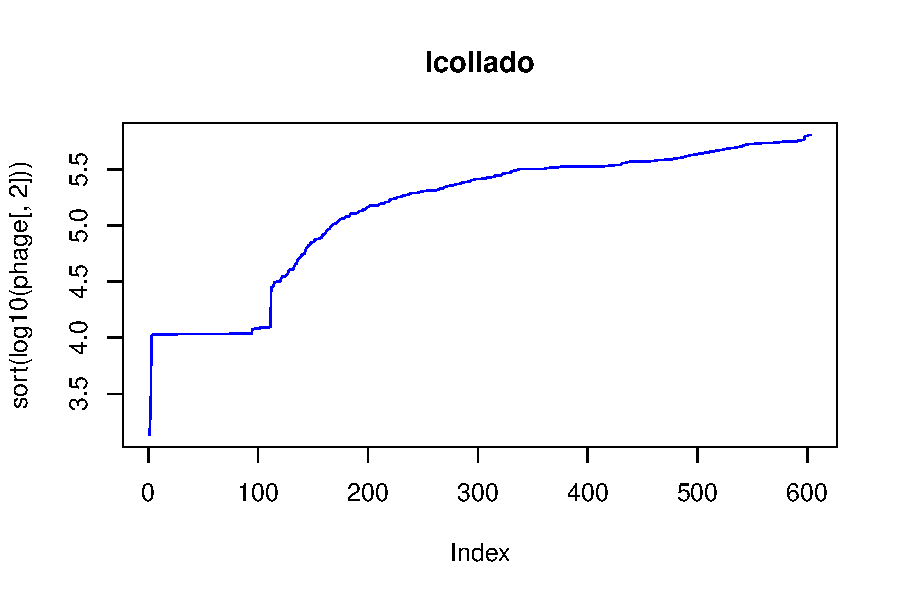
\includegraphics{plots/fig-007}
  \item Plot a histogram with a density line for the same data.  
\begin{Schunk}
\begin{Sinput}
> hist(phage[, 2], col = "light blue", 
+     prob = T)
> lines(density(phage[, 2]), col = "red")
\end{Sinput}
\end{Schunk}
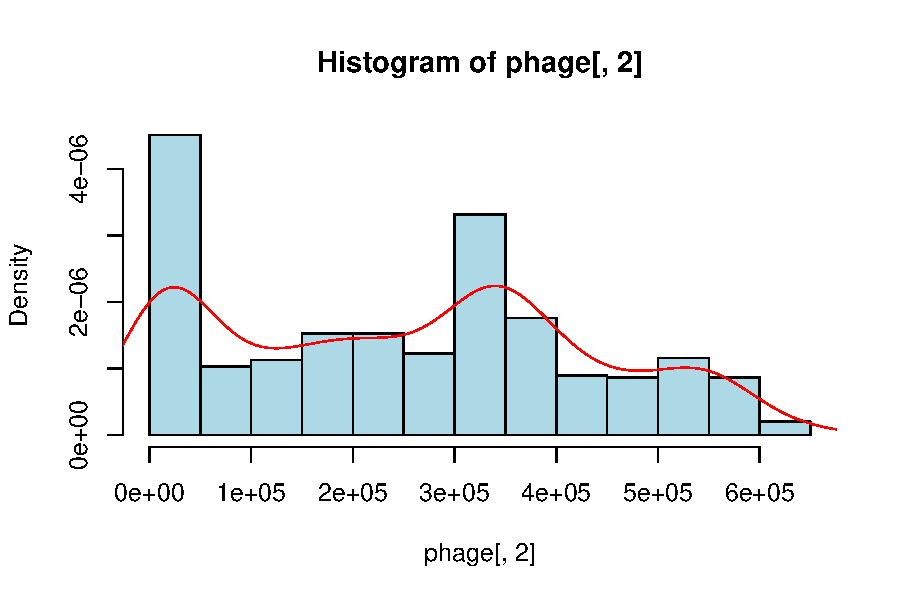
\includegraphics{plots/fig-008}
  \item Plot a boxplot for the differences between contigous sorted genomes. Meaning, 2nd smallest - smallest, 3rd smallest - 2nd smallest, etc.\footnote{You might want to use \pl{apropos} searching for diff\ldots}
\begin{Schunk}
\begin{Sinput}
> contig <- diff(sort(phage[, 2]))
> boxplot(contig, col = "forest green")
\end{Sinput}
\end{Schunk}
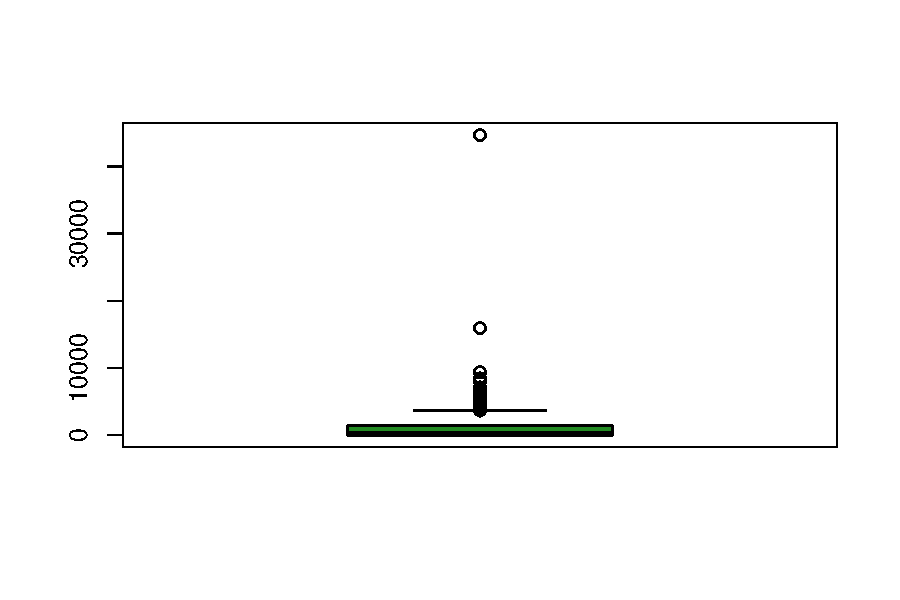
\includegraphics{plots/fig-009}
\begin{Schunk}
\begin{Sinput}
> contig <- diff(sort(log10(phage[, 
+     2])))
> boxplot(contig, col = "forest green")
> print("Boxplot without log10 was more useful")
\end{Sinput}
\begin{Soutput}
[1] "Boxplot without log10 was more useful"
\end{Soutput}
\end{Schunk}
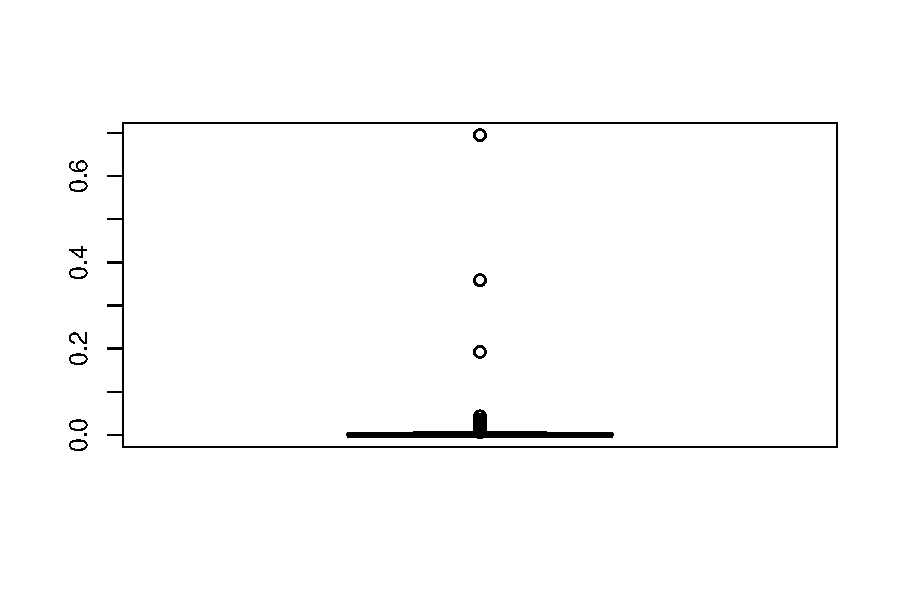
\includegraphics{plots/fig-010}
  \item Make a barplot showing the 10 biggest genomes. Include the names\footnote{They have to be redable} on the $x$ axis and every bar has to have a different color and/or density.\footnote{The \pl{which} function might be useful.}
\begin{Schunk}
\begin{Sinput}
> top <- sort(phage[, 2], decreasing = T)[1:10]
> names <- NULL
> for (i in 1:10) {
+     names <- c(names, phage[which(phage[, 
+         2] == top[i]), 1])
+ }
> barplot(top, col = rainbow(10), 
+     names.arg = phage[names, 1], 
+     cex.names = 0.5, las = 2, main = "lcollado")
\end{Sinput}
\end{Schunk}
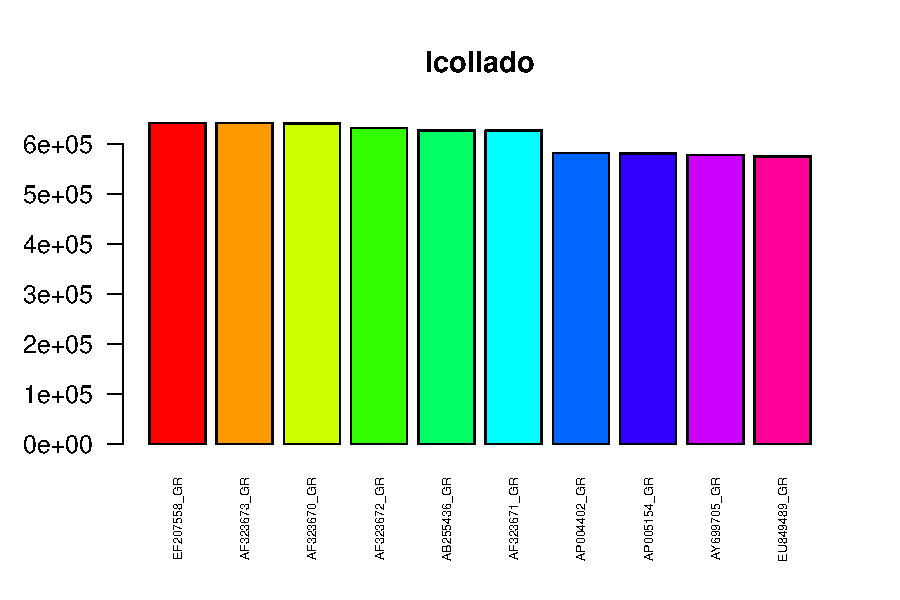
\includegraphics{plots/fig-011}
\begin{Schunk}
\begin{Sinput}
> barplot(log10(top), col = rainbow(10), 
+     names.arg = phage[names, 1], 
+     cex.names = 0.5, las = 2, main = "lcollado")
> print("Using log10 has almost no effect")
\end{Sinput}
\begin{Soutput}
[1] "Using log10 has almost no effect"
\end{Soutput}
\end{Schunk}
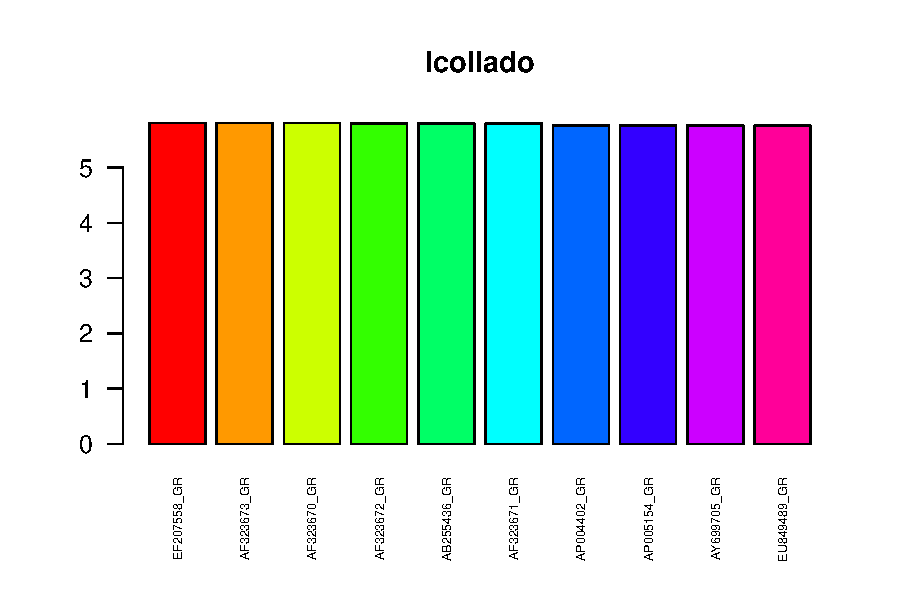
\includegraphics{plots/fig-012}
  \end{enumerate}
  \end{itemize}

\section{\pl{Apply} functions}
  \begin{enumerate}
  \item What is the mean genome size for every type of replicon (column 4)? You have an atomic vector and a factor so use \ldots
\begin{Schunk}
\begin{Sinput}
> tapply(phage[, 2], phage[, 4], 
+     mean)
\end{Sinput}
\begin{Soutput}
Chromosome  Segment L  Segment M 
  253726.3   106813.8   106813.8 
 Segment S 
  106813.8 
\end{Soutput}
\end{Schunk}
  \item Create a matrix \pl{mat} with 10 rows and 10 columns and 100 random uniform values from 1 to 10. Create your own function and apply it to every row so that every row will now sum 1 in your new matrix \pl{mat2}.
\begin{Schunk}
\begin{Sinput}
> mat <- matrix(runif(100, 1, 10), 
+     10, 10)
> mat2 <- t(sapply(1:10, function(x) {
+     mat[x, ]/sum(mat[x, ])
+ }))
> apply(mat2, 1, sum)
\end{Sinput}
\begin{Soutput}
 [1] 1 1 1 1 1 1 1 1 1 1
\end{Soutput}
\end{Schunk}
  \item Using the same matrix \pl{mat}, make the matrix \pl{mat3} with row sums equal to 1 using built in \pl{R} matrix functions. \pl{mat2} and \pl{mat3} should be the same.
\begin{Schunk}
\begin{Sinput}
> mat3 <- mat/rowSums(mat)
> rowSums(mat3)
\end{Sinput}
\begin{Soutput}
 [1] 1 1 1 1 1 1 1 1 1 1
\end{Soutput}
\end{Schunk}
  \end{enumerate}

\end{document}
